\documentclass{resume}

\begin{document}

\fontfamily{ppl}\selectfont

\noindent
\begin{tabularx}{\linewidth}{@{}m{0.8\textwidth} m{0.2\textwidth}@{}}
{
    \Large{Foma Shipilov} \newline
    \small{
        \clink{
            \href{mailto:foma@shipilov.ru}{foma@shipilov.ru}
            \textbf{·} 
            \href{https://t.me/foma2u}{@foma2u}
        } \newline
        Moscow, Russia
    }
} & 
{
    \hfill
    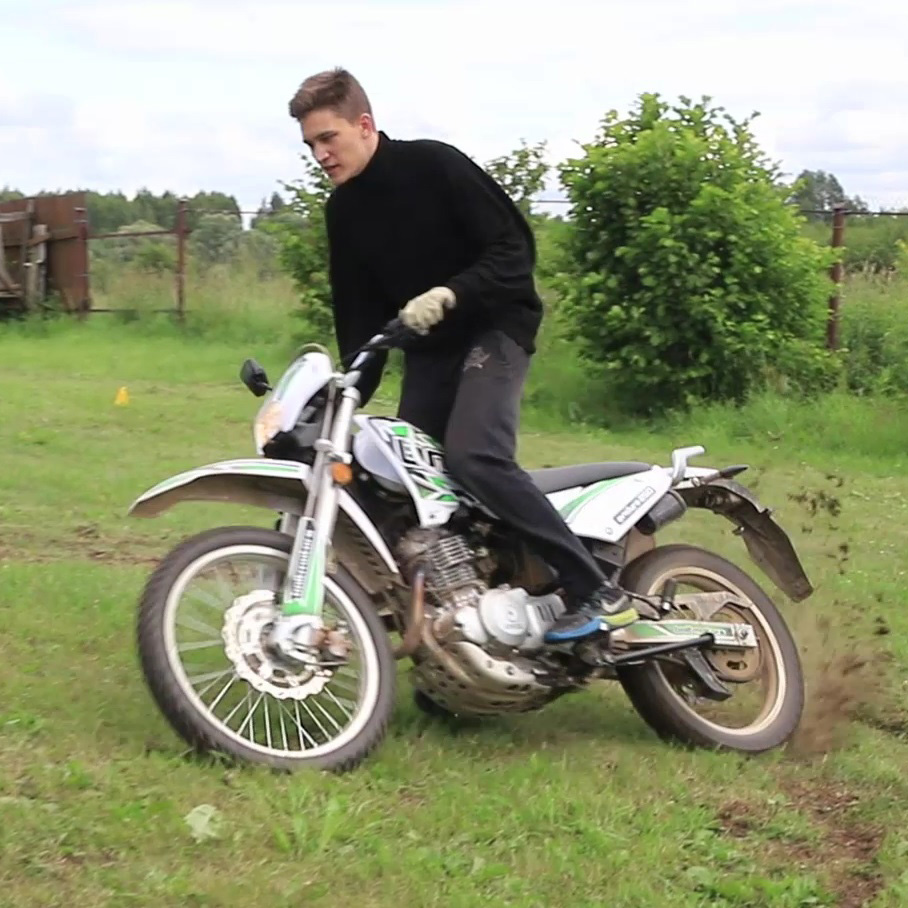
\includegraphics[width=2.8cm]{images/gr.jpg}
}
\end{tabularx}
\begin{center}
\begin{tabularx}{\linewidth}{@{}*{2}{X}@{}}
% left side %
{
    \csection{EXPERIENCE}{\small
        \begin{itemize}
            \item \frcontent{Huawei}{Assistant Engineer @ Noah’s Ark lab\vspace{0.2em}}{-- Remastered TV-series using GANs;\newline
            -- Developed non-linear CNN degradation model for super-resolution of real-world images.}{November 2020 -- September 2021}
            \item \frcontent{HSE University}{Intern-researcher @ Institute of Artificial Intelligence (LAMBDA)}{-- Deep learning applications for online filtering and reconstruction of aerogel detectors;\newline 
            \href{http://doi.org/10.1134/S106377882305037X}{What Machine Learning Can Do for Focusing Aerogel Detectors, Physics of Atomic Nuclei 86, 864 (2023)}}{November 2021 onwards}
            \item \frcontent{HSE University}{Teaching Assistant @ Faculty of Computer Science}{Teaching Instructor @ Deep Learning 1}{2020 -- 2024, September 2023 onwards}
        \end{itemize}
    }
    \csection{EDUCATION}{\small
        \begin{itemize}
            \item \frcontent{MSc Data Science (Studied in English)}{HSE University, Skoltech (MML joint programme)}{}{Currently undergoing}
            \item \frcontent{MSc + PhD Track, Computer Science}{HSE University}{}{Currently undergoing}
            \item \frcontent{BS Computer Science}{HSE University}{}{2023, Academic Honors Diploma}
        \end{itemize}
    }
    \csection{PROJECTS}{\small
        \begin{itemize}
            \item \frcontent{HiFi-GAN \clink{\href{https://github.com/xiyori/hw4_nv}{[github.com]}}}{Implementation of HiFi-GAN NeurIPS 2020 paper}{}{PyTorch}
            \item \frcontent{secHNet \clink{\href{https://github.com/xiyori/secHNet}{[github.com]}}}{PyTorch in Haskell from scratch}{}{Haskell, C}
            % \item \frcontent{Visual Turing \clink{\href{https://github.com/xiyori/turing_machine_emulator}{[github.com]}}}{Turing machine IDE in \textit{C++}}{}{}
            \vspace*{-3em}
        \end{itemize}
    }
} 
% end left side %
& 
% right side %
{
    \csection{SKILLS}{\small
        \begin{itemize}
            \item \textbf{ML \& Data Analysis} \newline
            {\footnotesize -- Computer vision, super-resolution, GANs, diffusion models, LLMs, deep learning for audio, deep Bayesian learning, mode connectivity \& permutation invariance\newline
            -- PyTorch, scikit-learn, OpenCV, NumPy, JAX, PySpark, Hadoop, Vowpal Wabbit}
            \item \textbf{Languages} \newline
            {\footnotesize Python, C, C++, C\#, Haskell, x86/ARM Assembly, HTML/CSS, ReactJS, Lua}
            \item \textbf{CI/CD \& Other} \newline
            {\footnotesize Docker, WandB, GitHub Actions, QuickCheck, GDB, Arch Linux, Shell}
        \end{itemize}
    }
	\csection{AWARDS \& RECOGNITION}{\small
		\begin{itemize}
            \item \frcontent{Yandex Scholarship}{HSE University}{Laureate}{2022}
			\item \frcontent{Vysshaya Liga, Math \& Informatics}{HSE University}{Degree I \& III Diploma}{2021, 2022}
			\item \frcontent{Ya Professional, Math Olympiad}{Yandex}{Prize-winner}{2021, 2022}
			% \item \frcontent{``Pokori Vorob'yovi Gori'' Math Olympiad}{Moscow State University}{Winner}{2019}
			\item \frcontent{Phystech, Math \& Physics Olympiads}{Moscow Institute of Physics and Technology}{Winner}{2019}
		\end{itemize}
	}
    %\csection{OTHER HIGHLIGHTS}{\small
    %    \begin{itemize}
    %        \item {\footnotesize Conducted biology studies within \textit{Structural and Functional Research of G-protein-coupled Cell Surface Receptors Using 3D Modeling} school project.}
    %    \end{itemize}
    %}
    \csection{HOBBIES \& INTERESTS}{\small
        \vspace{0.32cm}
        \begin{tabularx}{\linewidth}{@{}*{4}{>{\centering\arraybackslash}X}@{}}
            {\centering
            
\includegraphics[width=0.8cm]{images/skiing.png}
            } &
            {\centering
            
\includegraphics[width=0.8cm]{images/music.png}
            } & 
            {\centering
            
\includegraphics[width=0.8cm]{images/hyperspeedcube.png}
            } &
            {\centering
            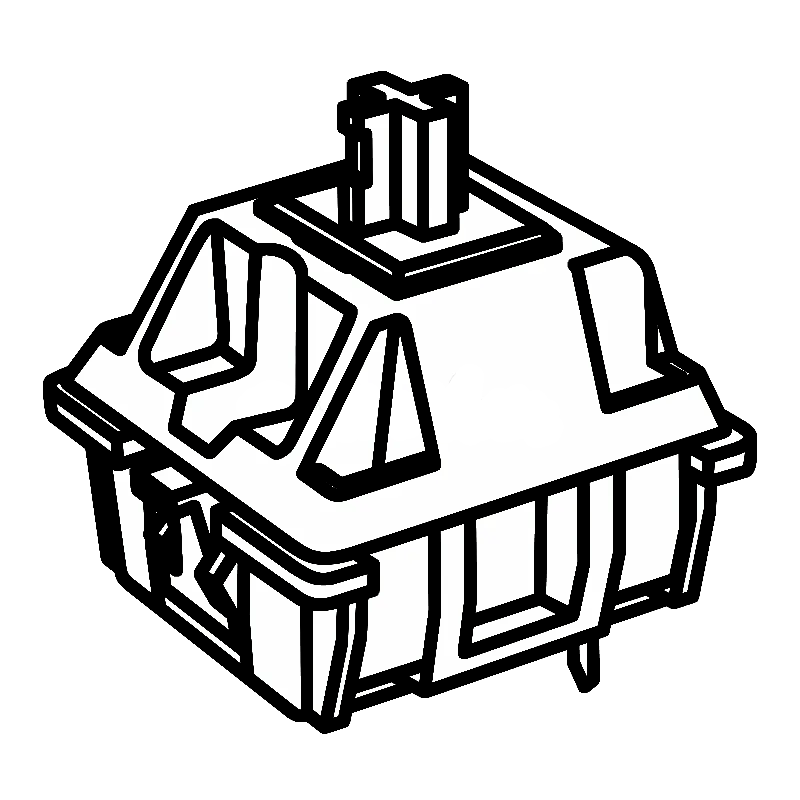
\includegraphics[width=0.8cm]{images/switch.png}
            } \\
            {\footnotesize Alpine skiing} & {\footnotesize Music production} & {\footnotesize Hypercubing} & {\footnotesize Custom keyboards}
        \end{tabularx}
    }
}
\end{tabularx}
\end{center}
\end{document}
